\documentclass{article}

\usepackage[english, russian]{babel}
\usepackage{geometry}
\usepackage{graphicx}
\usepackage{listings}
\usepackage{xcolor}
\usepackage[14pt]{extsizes}
\usepackage{amsmath}
\usepackage{setspace}
\usepackage{multirow}
\usepackage{tocloft}
\usepackage{indentfirst} 
\usepackage{lipsum}
\usepackage{caption}
\usepackage{cmap}
\usepackage[utf8]{inputenc}
\usepackage[T2A]{fontenc}

\captionsetup[figure]{name={Рисунок},labelsep=endash}
\captionsetup[table]{singlelinecheck=false, labelsep=endash}

\renewcommand{\cftsecleader}{\cftdotfill{\cftdotsep}}
\geometry{pdftex, left = 3cm, right = 1cm	, top = 2cm, bottom = 2cm}
\onehalfspacing

\setlength{\parindent}{1,25cm}
\lstdefinestyle{python}{
	language={Python},
	basicstyle=\footnotesize\ttfamily,
	frame=single,
	tabsize=4,	
	breaklines=true
}

\DeclareCaptionLabelSeparator{line}{\ --\ }
\DeclareCaptionFont{white}{\color{white}}
\DeclareCaptionFormat{listing}{\colorbox[cmyk]{0.43,0.35,0.35,0.01}{\parbox{\textwidth}{\hspace{15pt}#1#2#3}}}
\captionsetup[lstlisting]{
	singlelinecheck=false,
	labelsep=line
}

\begin{document}
\begin{titlepage}
	\newgeometry{pdftex, left=2cm, right=2cm, top=2.5cm, bottom=2.5cm}
	\fontsize{12pt}{12pt}\selectfont
	\noindent\begin{tabular}{|c|c|}	\hline
	\noindent\begin{minipage}{0.15\textwidth}
		
\includegraphics[width=\linewidth]{tools/logo.png}
	\end{minipage} &
	\noindent\begin{minipage}{0.85\textwidth}\centering
		\textbf{\newline Министерство науки и высшего образования Российской Федерации}\\
		\textbf{Федеральное государственное бюджетное образовательное учреждение высшего образования}\\
		\textbf{«Московский государственный технический университет имени Н.Э.~Баумана}\\
		\textbf{(национальный исследовательский университет)»}\\
		\textbf{(МГТУ им. Н.Э.~Баумана)}
	\end{minipage} \\
	\hline	\end{tabular}\newline\newline\newline
	\noindent ФАКУЛЬТЕТ \underline{«Информатика и системы управления»} \newline\newline
	\noindent КАФЕДРА \underline{«Программное обеспечение ЭВМ и информационные технологии»}\newline\newline\newline\newline\newline\newline

	\noindent\begin{minipage}{1.0\textwidth}\centering
		\Large\textbf{   ~~~ Лабораторная работа №4}\newline
		\textbf{по дисциплине «Анализ алгоритмов»}\newline\newline\newline\newline\newline
	\end{minipage}

	\noindent\textbf{Тема} \underline{Параллельные вычисления на основе нативных потоков}\newline\newline
	\textbf{Студент} \underline{Тузов Даниил Александрович}\newline\newline
	\textbf{Группа} \underline{ИУ7-52Б}\newline\newline
	\textbf{Преподаватель} \underline{Строганов Дмитрий Владимирович}
	
	\begin{center}
		\vfill
		Москва, \the\year ~г.
	\end{center}
	\restoregeometry
	\clearpage
\end{titlepage}

\renewcommand{\contentsname}{\begin{center}СОДЕРЖАНИЕ\end{center}} 
\tableofcontents
\setcounter{page}{2}
\clearpage

\begin{center}\section*{ВВЕДЕНИЕ}\end{center}
\addcontentsline{toc}{section}{ВВЕДЕНИЕ}

В 4 лабораторной работе рассматривается тема параллельных вычислений на основе нативных потоков.

Параллелизм описывает последовательности действий, которые происходят одновременно$^{[1]}$. Нередко в современных 
системах используется распараллеливание вычислений, которое может привести к росту временной эффективности программы.

Целью работы является разработка ПО, выполняющего скачивание страниц, содержащих рецепты с сайта$^{[4]}$.
Для достижения поставленной цели небходимо решить следующие задачи:
\begin{itemize}
	\item[--] рассмотреть структуру сайта;
	\item[--] разработать ПО, выполняющее скачивание страниц в однопоточном режиме;
	\item[--] разработать ПО, выполняющее скачивание страниц в многопоточном режиме;
	\item[--] провести исследование временных характеристик, написанных программ;
	\item[--] обосновать полученные результаты.
\end{itemize}


\clearpage\section{Входные и выходные данные}
Входными данными в этой программе является страница электронного ресурса, с которого необходимо скачать страницы, и
максимальное количество страниц, которые необходимо скачать. Выходными данными является директория с файлами,
содержащими html код страниц.

\clearpage\section{Преобразование входных данных в выходные}
Программа получает на вход ссылку на электронный ресурс и максимальное количество страниц выполняет код , указанный в
листинге~\ref{lst:script}:
\begin{lstlisting}[style=python, label=lst:script,caption=Скрипт на языке Python$^{[3]}$ для получения файла ссылок ля дальнейшей обработки]
import requests as re
import bs4

filename = "urls.txt"
url = "https://www.povareschka.ru"
list_catalogs = set()
list_links = set()

page = re.get(url)
bs = bs4.BeautifulSoup(page.content, 'html.parser')
for groups in bs.find_all('menu')[1:-2]:
    for link in groups.find_all('a'):
        ref = link.get('href')
        if 'recepty' in ref:
            list_catalogs.add(url + ref)

for part in list_catalogs:
    page = re.get(part)
    bs = bs4.BeautifulSoup(page.content, 'html.parser')
    for groups in bs.find_all('main'):
        for link in groups.find_all('a'):
            ref = link.get('href')
            if 'recepty' in ref:
                list_links.add(url + ref)

f = open(filename, "w")
for i in list_links:
    f.write(i + '\n')
\end{lstlisting}

В результате работы формируется файл, содержащий в каждой строке ссылку на страницу с рецептом. В дальнейшем этот файл
подается на вход программе на языке C++, которая выполняет сохранение страниц в файлы и формирует итоговую директорию.

\clearpage\section{Тестирование}
При тестировании программы на вход подавался файл с единственной ссылкой на рецепт. В результате работы 
формировалась директория с единственным файлом, содержащим html код заданной страницы. На следующем этапе 
выполнялось сравнение кода элемента искомой страницы с кодом в полученном файле.

Тестирование выполнялось как для однопоточной программы, так и для многопоточной.

В многопоточной программе так же учитывалось количество создаваемых потоков.

\clearpage\section{Примеры работы программы}
На рисунках~\ref{pict:in}~-~\ref{pict:out} приведен пример работы программы.
	
\begin{figure}[h]
	\centering
	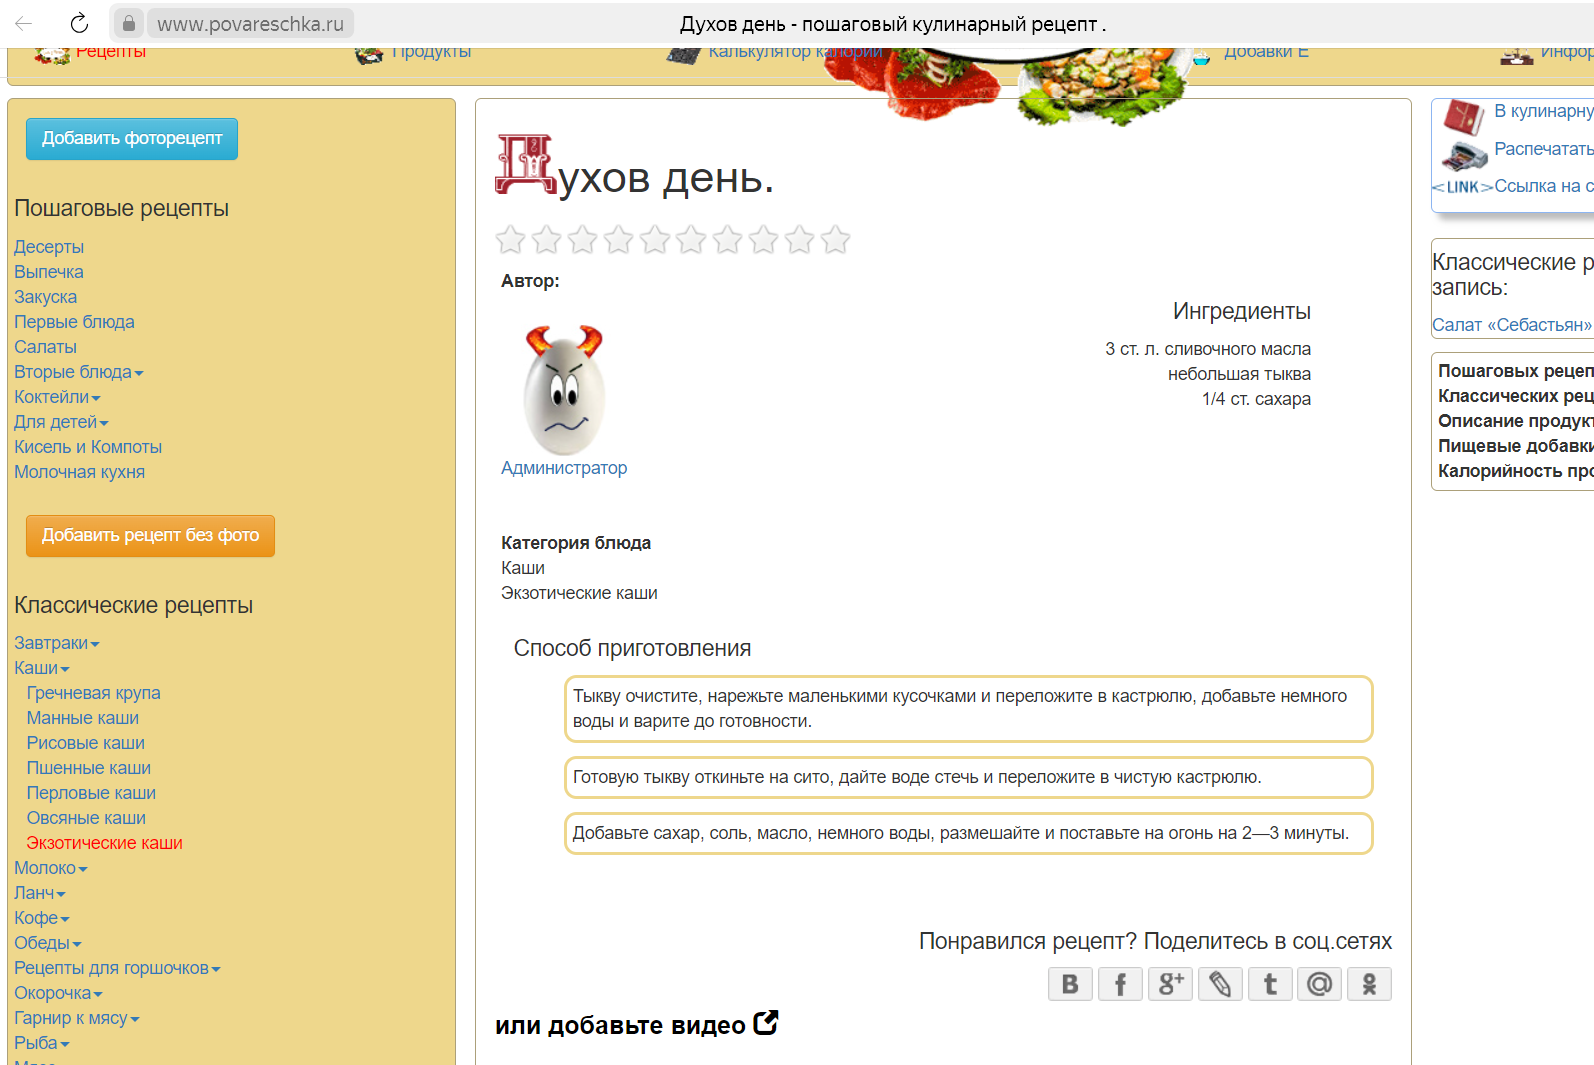
\includegraphics[scale=0.4]{tools/in.png}
	\caption{Страница сайта, с которой необходимо скачать рецепт}
	\label{pict:in}
\end{figure}

\begin{figure}[h]
	\centering
	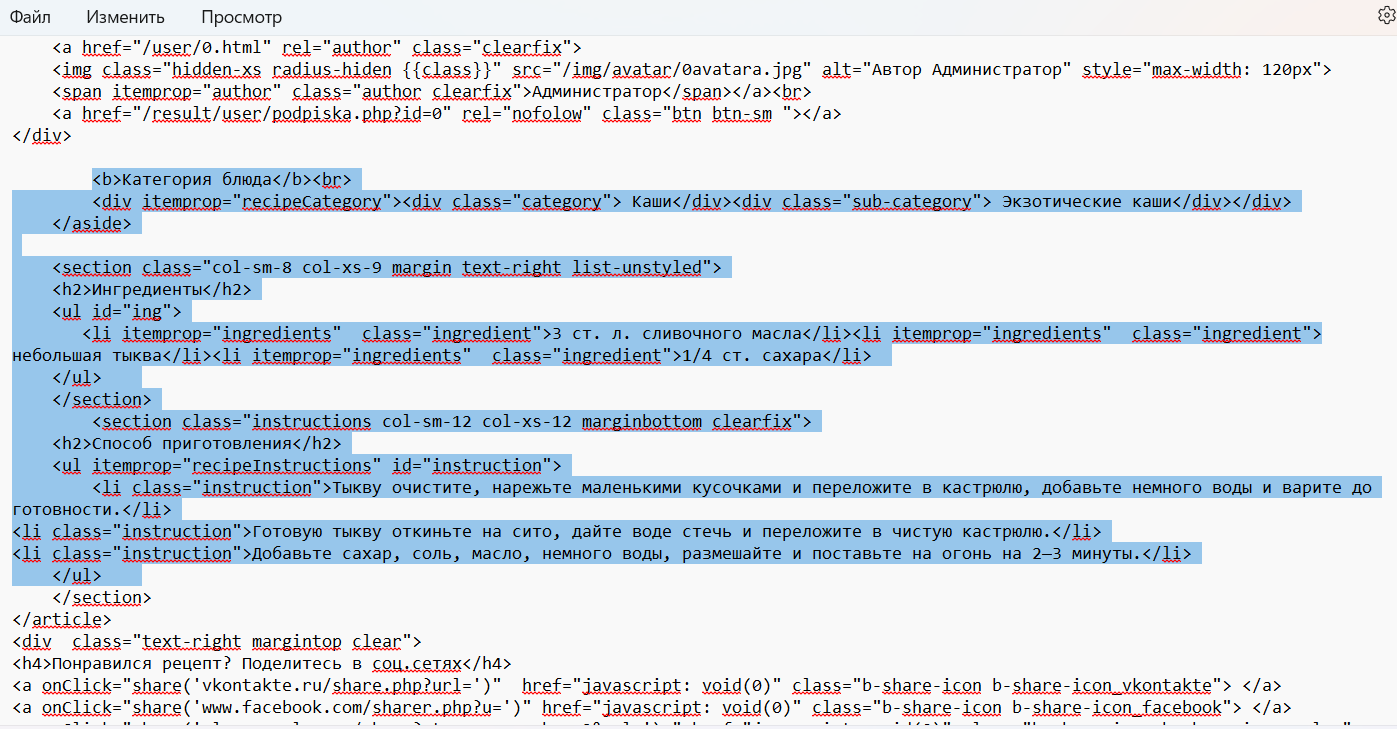
\includegraphics[scale=0.4]{tools/out.png}
	\caption{Файл, содержащий html-код страницы}
	\label{pict:out}
\end{figure}

\clearpage\section{Описание исследования}
В ходе исследования сравнивалось время работы программ с различным количеством потоков: 1, 2, 4, 8, 16, 32, 48, 64.

Все замеры проводились на ЭВМ, характеристики которой приведены ниже:
\begin{itemize}
	\item[--] процессор -- 12th Gen Intel(R) Core(TM) i5-12450H   2.00 ГГц;
	\item[--] оперативная память -- 16,0 ГБ;
	\item[--] тип системы -- 64-разрядная операционная система, процессор x64;
	\item[--] операционная система -- Windows 11;
	\item[--] версия ОС -- 23H2;
	\item[--] 12 логических ядер.
\end{itemize}

Для получения результата на вход подавалось 200 ссылок. Проводилось 20 замеров, результаты усреднялись.

Полученные результаты представлены на рисунке~\ref{time} и в таблице~\ref{table}:
\begin{figure}[h]
	\centering
	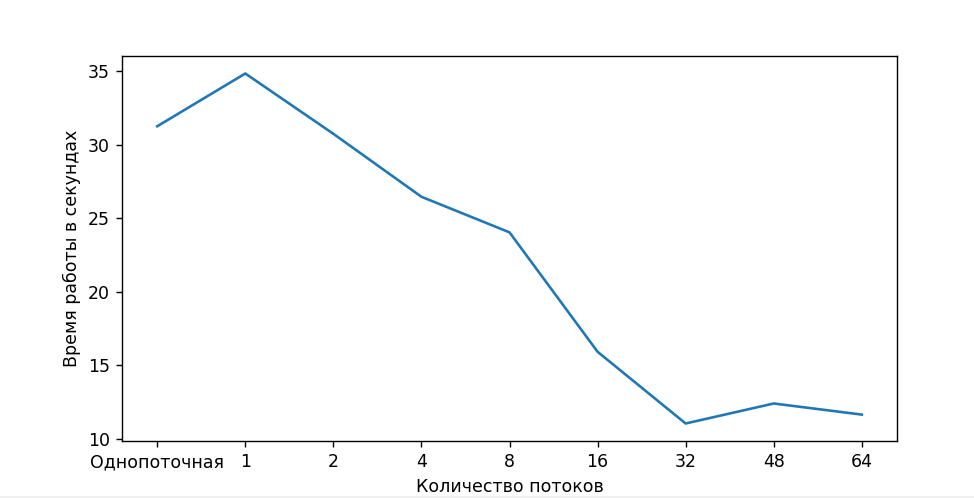
\includegraphics[scale=0.8]{tools/time.png}
	\caption{Время работы программы}
	\label{time}
\end{figure}

\clearpage\begin{table}[h]
	\begin{center}
	\caption{\label{table} Время работы программы}
	\begin{tabular}{|c|c|}
		\hline
		Количество потоков & Время работы, с 
		\\ \hline
		\multicolumn{2}{|c|}{Однопоточная реализация} 
		\\ \hline
		1 & 31.24 
		\\ \hline
		\multicolumn{2}{|c|}{Многопоточная реализация} 
		\\ \hline
		1 & 34.82 
		\\ \hline
		2 & 30.73 
		\\ \hline
		4 & 26.45 
		\\ \hline
		8 & 24.03 
		\\ \hline
		16 & 15.92
		\\ \hline
		32 & 11.05
		\\ \hline
		48 & 12.4
		\\ \hline
		64 & 11.66
		\\ \hline
	\end{tabular}
	\end{center}
\end{table}

В результате исследования можно сделать вывод, что использование параллельных вычислений может ускорить программу.
Чем больше потоков, тем больше ускорение, однако с определенного момента выигрыш становится незначительным.

\clearpage\begin{center}\section*{ЗАКЛЮЧЕНИЕ}\end{center}
\addcontentsline{toc}{section}{ЗАКЛЮЧЕНИЕ}
В ходе выполнения лабораторной работы поставленная цель была достигнута, а также были решены следующие задачи:
\begin{enumerate}
	\item рассмотрена структура сайта;
	\item написан скрипт на языке $Python$, который скачивает ссылки рецептов с заданного сайта;
	\item написана однопоточная и многопоточная программы, скачивающие рецепты;
	\item проведено сравнение временных характеристик работы программ: выявлено, что использование параллельных
вычислений ускоряет программу, однако с определенного момента это ускорение незначительно;
	\item обоснованы полученные результаты и сделан вывод.
\end{enumerate} 

\clearpage\begin{center}\section*{\normalsizeСПИСОК ИСПОЛЬЗОВАННЫХ ИСТОЧНИКОВ}\end{center}
\addcontentsline{toc}{section}{СПИСОК ИСПОЛЬЗОВАННЫХ ИСТОЧНИКОВ}
\begin{enumerate}
	\item Энтони Уильямс, C++. Практика многопоточного программирования. / Второе издание
	\item Ковалев, Введение в многопоточность / [Электронный ресурс] // Режим доступа: https://rekovalev.site/multithreading-3-cpp/\#threads-create
	\item Язык Python / [Электронный ресурс] // Режим доступа: https://docs.python\\.org/3/index.html
	\item Кулинарные рецепты / [Электронный ресурс] // Режим доступа: https://www\\.povareschka.ru/
 \end{enumerate}

\end{document}